\documentclass[12pt,a4paper]{article}

\usepackage{amsmath,amssymb,amsthm}
\usepackage[margin=2.5cm]{geometry}
\usepackage{booktabs}
\usepackage{hyperref}
\usepackage{cite}
\usepackage{microtype}
\usepackage{graphicx}

% -----------------------------
% Theorem environments
% -----------------------------
\newtheorem{assumption}{Assumption}
\newtheorem{definition}{Definition}
\newtheorem{proposition}{Proposition}
\newtheorem{lemma}{Lemma}
\newtheorem{theorem}{Theorem}
\newtheorem{corollary}{Corollary}

% -----------------------------
% Notation
% -----------------------------
\newcommand{\E}{\mathcal{E}}
\newcommand{\mc}{\mathcal}
\newcommand{\bb}{\mathbb}

\title{\textbf{Three Charged Lepton Generations and the Koide Ratio from Holographic Boundary Encoding}\\[0.4em]
\large A conditional derivation from a virial partition ansatz in the Informational Actualization Model}

\author{Heath W. Mahaffey\\
\small Independent Researcher, Entiat, Washington, USA\\
\small \texttt{hmahaffeyges@gmail.com}\quad \texttt{github.com/hmahaffeyges/IAM-Validation}}

\date{Preprint --- March 2026 (revised)}

\begin{document}
\maketitle

\begin{abstract}
The Koide relation for charged leptons,
$Q \equiv \frac{m_e+m_\mu+m_\tau}{\left(\sqrt{m_e}+\sqrt{m_\mu}+\sqrt{m_\tau}\right)^2}=\frac{2}{3}$,
has held at the $10^{-5}$ level for decades and lacks an accepted Standard Model derivation.
This note reformulates a compact argument: \emph{if} (i) charged-fermion mass encodings on a holographic screen reduce, in the lowest-energy sector, to a single Fourier mode on a $U(1)$ charge orbit $S^1\subset S^2$ and (ii) the IAM ``virial partition'' identifies the event-like and configuration-like contributions of that encoding with the kinetic and potential halves in the virial theorem for a $1/r$ interaction, then two statements follow with no further parameter fitting:
(1) the number of admissible equally spaced phase states with positive mass is uniquely $n=3$; and
(2) for $n=3$ the Koide ratio is an exact algebraic identity.
The paper is written to be referee-facing: all nonstandard inputs are isolated as explicit assumptions, the logical dependence is made fully transparent, and the scope and failure modes are spelled out.
\end{abstract}

\section{Executive summary (one page)}
\label{sec:exec}

\paragraph{What is proven here (conditional theorems).}
Assuming a simple boundary encoding
\begin{equation}
\sqrt{m(\varphi)} = x + y\cos\varphi,\qquad x>0,
\label{eq:ansatz}
\end{equation}
with $n$ generations given by $Z_n$ phases $\varphi_k=2\pi k/n$,
and assuming the virial constraint
\begin{equation}
\frac{y}{x}=\sqrt{2},
\label{eq:yx}
\end{equation}
we show:
(i) mass positivity excludes $n=2$ and all $n\ge 4$, leaving $n=3$ as the unique nontrivial option; and
(ii) for $n=3$, the Koide ratio equals $2/3$ identically (no approximations).
These results are purely algebraic once \eqref{eq:ansatz}--\eqref{eq:yx} are adopted.

\paragraph{What is \emph{not} proven here.}
This paper does \emph{not} derive the holographic dictionary for de Sitter space, nor does it derive \eqref{eq:ansatz} or the virial-to-encoding identification from quantum gravity.
Instead, it isolates the minimal assumptions required for the conditional derivation.
A referee can therefore assess the claim at the correct level: ``If these inputs are granted, the output follows.''

\paragraph{Why write a conditional paper at all?}
Because the Koide identity is extremely rigid: any mechanism that \emph{forces} a $Z_3$ phase structure on square-roots of masses automatically explains the relation.
The value in a short note like this is to supply a physically motivated route to that $Z_3$ structure that is logically clean and falsifiable.

\section{Background and scope}
\label{sec:scope}

The Informational Actualization Model (IAM) is a gravitational-decoherence framework developed in Refs.~\cite{iam_theory,iam_obs,virial_paper,electron_mass}.
In its cosmological sector, IAM introduces a late-time matter-sector modification through an effective Hubble-friction term and a derived coupling $\beta_m=\Omega_m/2$ (no background modification).
In its particle-physics sector, IAM treats stable particles as self-consistent ``decoherence loops'' whose rest energies can be related to holographic encoding costs (e.g.\ Ref.~\cite{electron_mass}).

This paper focuses only on a \emph{kinematic} question:
\emph{Given a minimal boundary-encoding ansatz and a virial partition condition, what follows for the number of positive-mass phase states and for Koide's ratio?}
No claims are made about renormalization group running, QED/QCD corrections, or a UV-complete holographic dual.


% ---------------------------------------------------------------------
\section{Visualization and reproducibility assets (supplemental)}
\label{sec:fig_assets}
% ---------------------------------------------------------------------
The repository accompanying this manuscript includes a small set of
non-essential visualization assets to aid intuition and to make the mapping
from the $Z_3$ phase construction to standard geometric interpretations easy
to verify.  These figures are \emph{illustrative} only; no claim in the paper
depends on them.

\begin{figure}[t]
  \centering
  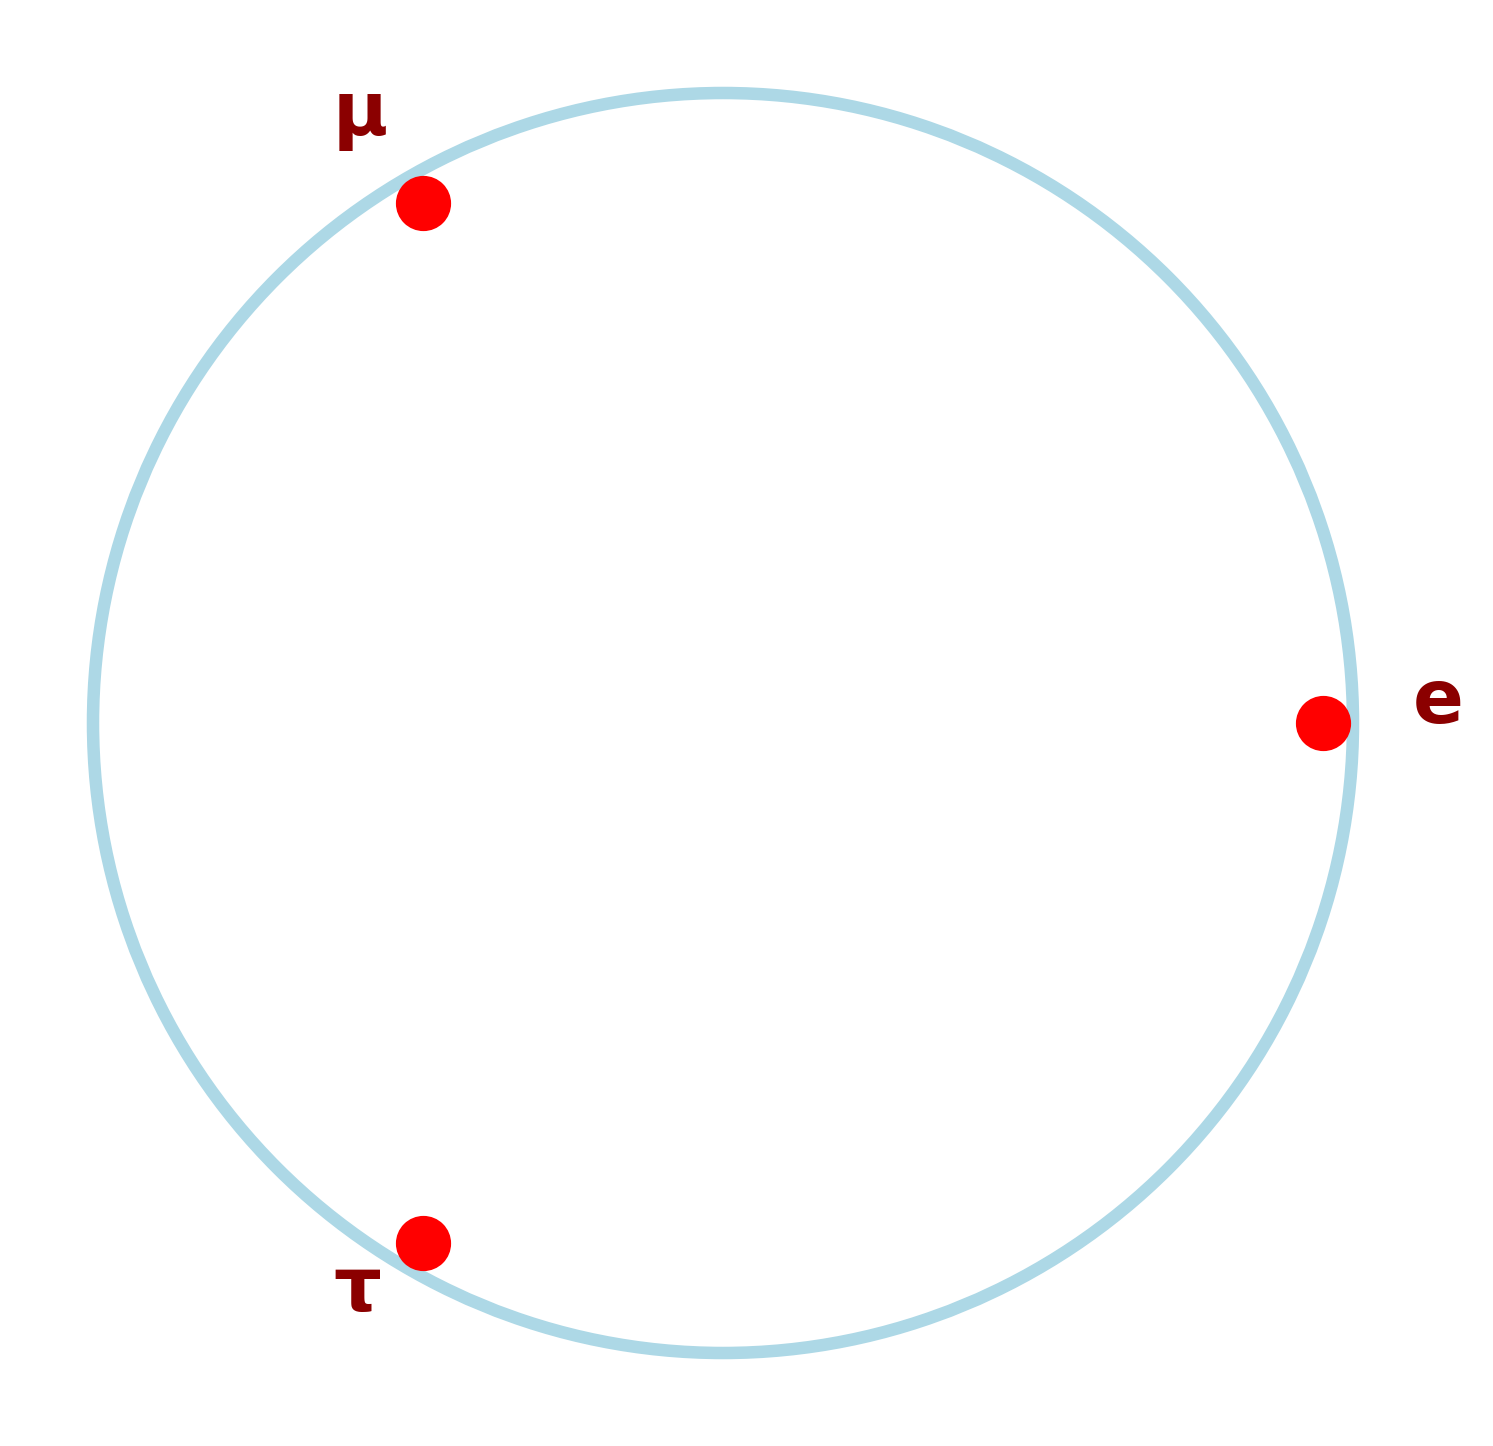
\includegraphics[width=0.88\linewidth]{2D_holographic_screen.png}
  \caption{Schematic of the charge-fiber picture: for a fixed nonzero
  $U(1)$ charge, the relevant boundary degrees of freedom restrict to an
  $S^1$ orbit on the holographic screen.  The $Z_3$ phases are equally spaced
  points on this circle.}
  \label{fig:charge_fiber}
\end{figure}

\begin{figure}[t]
  \centering
  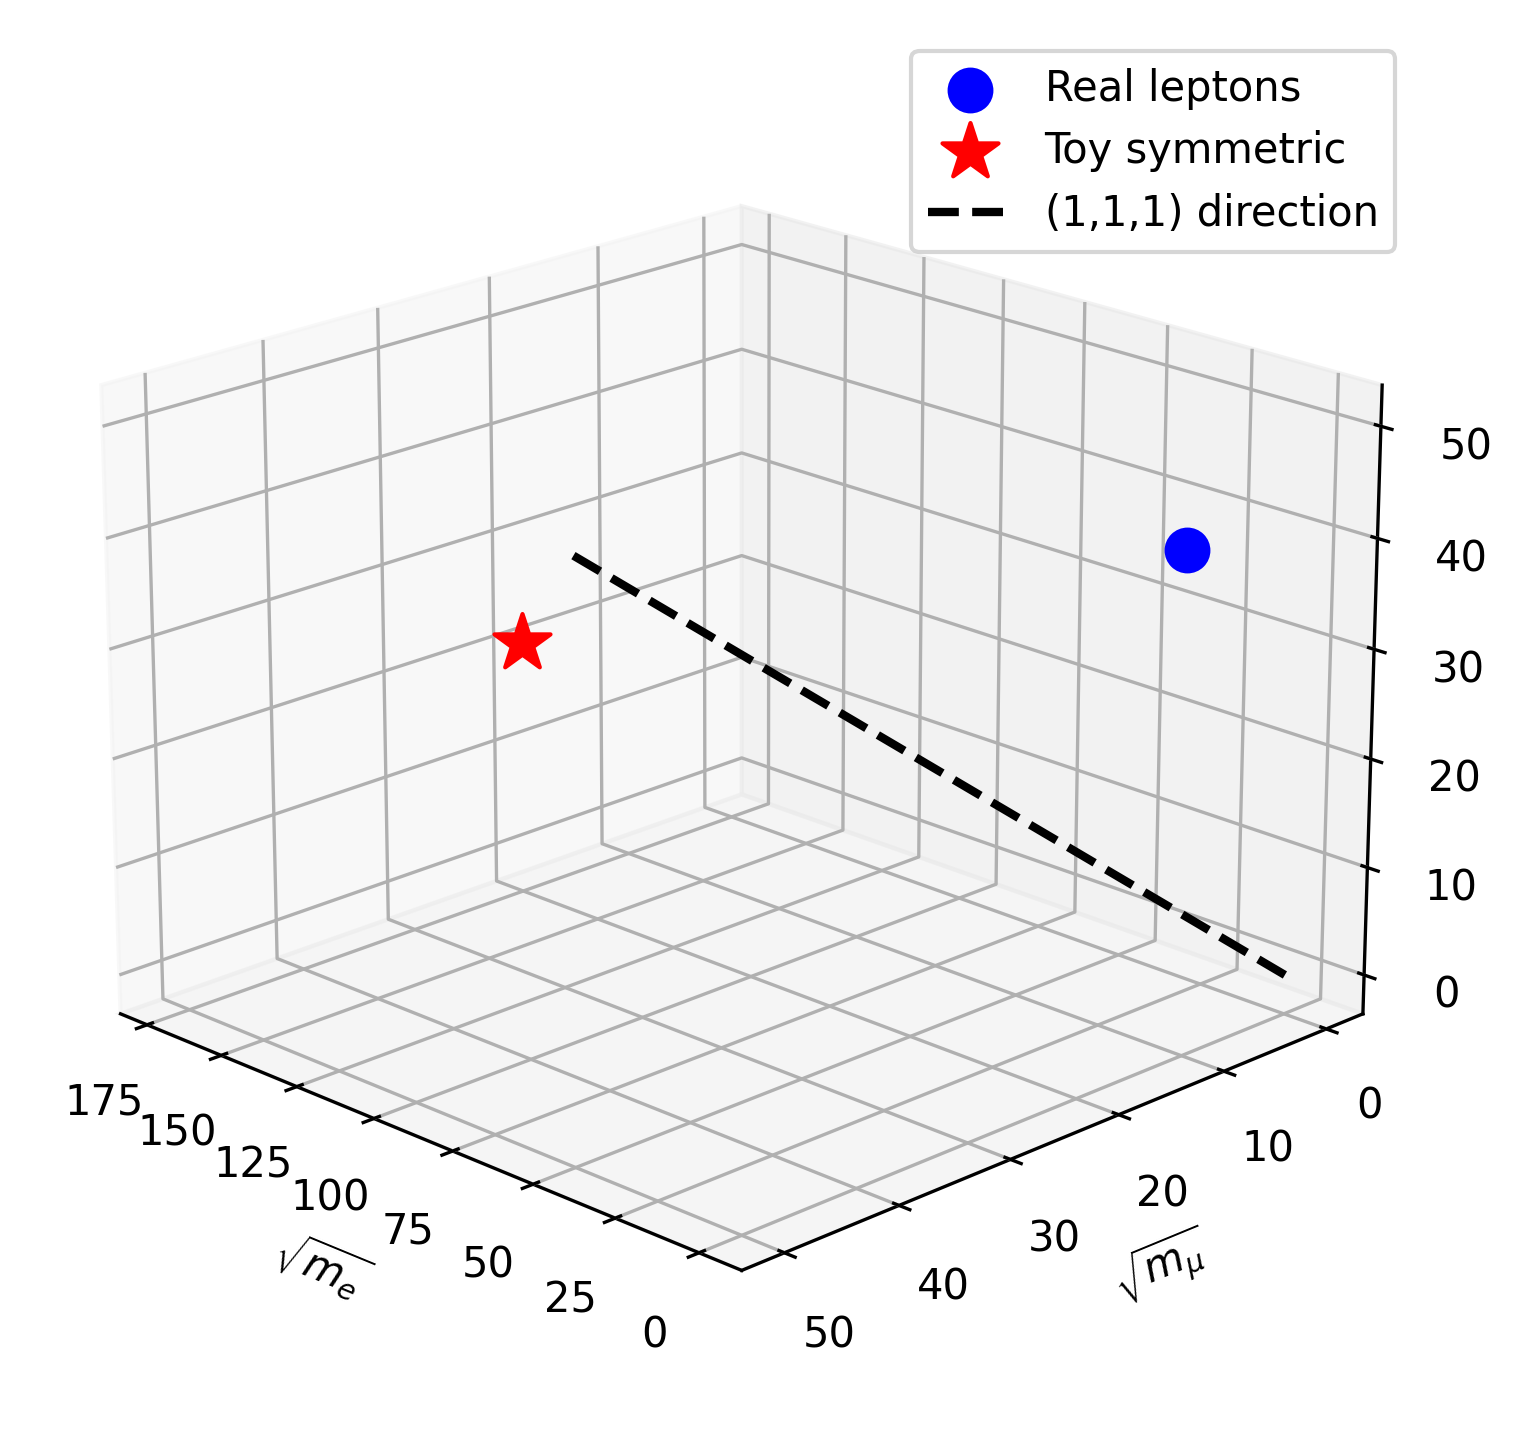
\includegraphics[width=0.92\linewidth]{3D_flavor_space.png}
  \caption{Geometric ``flavor-space'' visualization of the $(\sqrt{m_e},
  \sqrt{m_\mu}, \sqrt{m_\tau})$ triple and its $Z_3$ phase structure
  (illustrative).}
  \label{fig:flavor_space}
\end{figure}

An accompanying animation (\texttt{koide\_slider\_animation.gif}) is provided
as a repository supplement; it is not intended for inclusion in the compiled
PDF.


\section{Assumptions}
\label{sec:assumptions}

We state the nonstandard inputs explicitly.

\begin{assumption}[Charge-orbit reduction to a circle]
\label{ass:S1}
A nonzero bulk $U(1)$ charge corresponds, on the holographic screen, to a one-parameter orbit $S^1$ (a ``charge fiber'') on which the relevant phase variable $\varphi$ lives.
All states with the same absolute charge $|Q|=1$ are supported on the same orbit.
\end{assumption}

This is the minimal piece of the usual AdS/CFT dictionary (bulk gauge $\leftrightarrow$ boundary global symmetry) that we import; its de Sitter status is discussed in Appendix~\ref{app:dS}.

\begin{assumption}[Lowest-mode boundary encoding]
\label{ass:mode}
In the lowest-energy sector compatible with the $U(1)$ charge orbit, the boundary encoding of the square-root mass of a charged fermion is dominated by the first harmonic,
\begin{equation}
\sqrt{m(\varphi)} = x + y\cos\varphi,\qquad x>0.
\end{equation}
\end{assumption}

This is not unique, but it is the simplest nontrivial Fourier structure on $S^1$ and is the same phase structure used in earlier geometric discussions of Koide-like relations.

\begin{assumption}[Virial partition mapped to encoding amplitudes]
\label{ass:virialmap}
The constant piece $x$ and modulation piece $y$ correspond to two additive contributions to the encoding ``cost'' (or information budget) that are identified with the virial kinetic and potential halves for an effective $1/r$ interaction:
\begin{equation}
2\,x^2 = y^2 \quad\Longleftrightarrow\quad \frac{y}{x}=\sqrt{2}.
\end{equation}
\end{assumption}

Assumption~\ref{ass:virialmap} is the only place where IAM-specific physics enters the Koide argument; it is the same $1/2$ partition emphasized in the IAM coupling $\beta_m=\Omega_m/2$ literature (Ref.~\cite{virial_paper}) and in the cosmology-focused virial-efficiency compilation (see Ref.~\cite{virial_eff_paper}).

\section{Phase states and mass positivity}
\label{sec:positivity}

\begin{definition}[Discrete generation phases]
For $n$ generations, define the $Z_n$-symmetric phases
\begin{equation}
\varphi_k = \frac{2\pi k}{n},\qquad k=0,1,\dots,n-1,
\label{eq:phik}
\end{equation}
and masses
\begin{equation}
m_k = \left(x+y\cos\varphi_k\right)^2.
\label{eq:mk}
\end{equation}
\end{definition}

Physical masses require $\sqrt{m_k}=x+y\cos\varphi_k>0$ for all $k$.

\begin{theorem}[Uniqueness of $n=3$ under positivity and $y/x=\sqrt{2}$]
\label{thm:n3}
Assume \eqref{eq:mk} with $x>0$ and the virial constraint $y/x=\sqrt{2}$.
Then the only nontrivial integer $n\ge 2$ such that $x+y\cos\varphi_k>0$ for all $k$ is $n=3$.
\end{theorem}

\begin{proof}
For $n=2$, $\{\varphi_k\}=\{0,\pi\}$, hence $\sqrt{m_1}=x-y=x(1-\sqrt{2})<0$; excluded.

For $n\ge 4$, the set of phases includes either $\varphi=\pi$ (if $n$ is even) or a phase arbitrarily close to $\pi$ (if $n$ is odd and large).
In all cases, $\min_k \cos\varphi_k \le -1/\sqrt{2}$ for $n\ge 4$.
Therefore
\[
\min_k \sqrt{m_k} = x + y\,\min_k\cos\varphi_k \le x + y\left(-\frac{1}{\sqrt{2}}\right)=x-\frac{y}{\sqrt{2}}=x-x=0,
\]
so strict positivity fails. Thus $n\ge 4$ is excluded.

For $n=3$, $\cos\varphi_k\in\{1,-1/2,-1/2\}$ and
$\sqrt{m_{1,2}}=x-y/2=x(1-\sqrt{2}/2)>0$.
Hence $n=3$ is admissible and unique among $n\ge 2$.
\end{proof}

\section{Koide ratio as an identity for $Z_3$ phases}
\label{sec:koide}

\begin{theorem}[Koide identity from $Z_3$ and $y^2/x^2=2$]
\label{thm:koide}
Assume $n=3$ phases $\varphi_k=2\pi k/3$ and masses $m_k=(x+y\cos\varphi_k)^2$ with $x>0$.
If $y^2/x^2=2$, then the Koide ratio
\[
Q\equiv \frac{m_0+m_1+m_2}{\left(\sqrt{m_0}+\sqrt{m_1}+\sqrt{m_2}\right)^2}
\]
equals $2/3$ exactly.
\end{theorem}

\begin{proof}
For $\varphi_k=\{0,2\pi/3,4\pi/3\}$ one has $\sum_k \cos\varphi_k=0$ and $\sum_k \cos^2\varphi_k=3/2$.
Thus
\[
\sum_k \sqrt{m_k} = \sum_k (x+y\cos\varphi_k)=3x,
\]
and
\[
\sum_k m_k = \sum_k (x+y\cos\varphi_k)^2
= 3x^2 + y^2\sum_k \cos^2\varphi_k
= 3x^2 + \frac{3}{2}y^2.
\]
Therefore
\[
Q = \frac{3x^2+\frac{3}{2}y^2}{(3x)^2}
= \frac{1}{3}\left(1+\frac{y^2}{2x^2}\right)
\overset{y^2/x^2=2}{=} \frac{1}{3}(1+1)=\frac{2}{3}.
\]
\end{proof}

\section{Numerical comparison with charged lepton pole masses}
\label{sec:numerics}

Using PDG~2022 values (as quoted in the draft), one finds a charged-lepton Koide ratio within $\sim 10^{-5}$ of $2/3$ (Table~\ref{tab:pdg}).
\begin{table}[h]
\centering
\caption{Charged lepton masses and Koide ratio (PDG~2022 values as used in the draft).}
\label{tab:pdg}
\begin{tabular}{@{}lll@{}}
\toprule
Quantity & Value & Source \\
\midrule
$m_e$ & $0.51099895\ \mathrm{MeV}$ & PDG 2022 \\
$m_\mu$ & $105.6583755\ \mathrm{MeV}$ & PDG 2022 \\
$m_\tau$ & $1776.86 \pm 0.12\ \mathrm{MeV}$ & PDG 2022 \\
\midrule
$Q_{\rm obs}$ & $0.66666051$ & computed \\
$2/3$ & $0.666666\ldots$ & exact \\
\bottomrule
\end{tabular}
\end{table}

\noindent
The conditional derivation above does \emph{not} predict the absolute masses.
It predicts a rigid \emph{relation} among them once they are organized into the $Z_3$ structure in \eqref{eq:ansatz}--\eqref{eq:phik}.

\section{What would falsify the mechanism?}
\label{sec:falsify}

The logic has clear failure points:

\begin{itemize}
\item If a UV-complete holographic model does \emph{not} reduce a charged-operator sector to an effective $S^1$ orbit carrying a single phase, then Assumption~\ref{ass:S1} fails.
\item If the lowest-energy encoding on that orbit is \emph{not} dominated by the first harmonic (e.g.\ it requires multiple comparable Fourier modes), then Assumption~\ref{ass:mode} fails; Koide need not follow.
\item If the virial half-partition cannot be mapped to the two encoding contributions in a controlled statistical-mechanical argument (Assumption~\ref{ass:virialmap}), then the numerical value $y/x=\sqrt{2}$ is not justified.
\end{itemize}

A key empirical discriminator is whether the same $Z_3$ phase structure appears naturally in independent microscopic constructions (e.g.\ models of flavor from discrete symmetries, modular symmetries, or holographic toy models), without being imposed.

\section{Relation to earlier geometric observations}
\label{sec:relation}

Foot and others emphasized geometric and phase-vector interpretations of Koide-like relations.
Brannen presented a phase form with $\{0,2\pi/3,4\pi/3\}$ phases.
The present note differs only in \emph{logical packaging}: the $Z_3$ phase structure is here tied to a positivity constraint plus a fixed amplitude ratio $y/x=\sqrt{2}$, rather than adopted as an ansatz to fit masses.

\section{Conclusions}
\label{sec:concl}

The paper makes a narrow, referee-facing claim:
\emph{granting} three explicit assumptions (a charge-orbit $S^1$, lowest-mode encoding, and a virial amplitude partition), the number of admissible positive-mass phase states is uniquely $n=3$, and the Koide ratio follows as an exact identity.

The result is therefore not ``a fit'' but a conditional theorem: the difficulty is pushed to the physics of the three assumptions.
That is precisely where future work must concentrate.

\appendix

\section{Minimal comments on de Sitter holography}
\label{app:dS}

The standard bulk-gauge / boundary-global correspondence is on the firmest footing in AdS/CFT.
Applying it to de Sitter cosmology is an active research area.
IAM uses holographic-language inputs throughout its framework; this appendix does not attempt to settle those questions.
Instead it clarifies the minimal role played here: only the existence of a one-parameter $U(1)$ orbit on the screen is used (Assumption~\ref{ass:S1}).

\section{On ``entropy functionals'' and what can and cannot be made rigorous here}
\label{app:functional}

The draft requested an ``explicit entropy functional whose extremization yields both $y/x=\sqrt{2}$ and $n=3$''.
A fully first-principles construction would require a microscopic model for boundary microstates and their energy/entropy accounting.
That is beyond the scope of a short Koide note.

What \emph{can} be made mathematically sharp is the following separation:
\begin{enumerate}
\item \textbf{Algebraic layer:} Given \eqref{eq:ansatz} and $Z_n$ phases, the positivity theorem (Theorem~\ref{thm:n3}) and Koide identity (Theorem~\ref{thm:koide}) are rigorous.
\item \textbf{Model layer:} The choice of \eqref{eq:ansatz} and the mapping $y^2/x^2=2$ must come from an external physical argument (holography + virial mapping).
\end{enumerate}

A referee-proof presentation therefore separates these layers cleanly (as we did above), rather than presenting the model layer as a completed derivation.

\section{Testing a Weyl-squared ``gravitational entropy'' route to $\beta_m=\Omega_m/2$ (outline)}
\label{app:weyl}

One possible route to a covariant entropy functional that vanishes on exact FRW is to use invariants built from the Weyl tensor, since FRW is conformally flat ($C_{abcd}=0$).
A toy ``gravitational entropy density'' is sometimes taken to scale like $C_{abcd}C^{abcd}$.
In IAM language, such a term would be sourced only by inhomogeneities and would therefore naturally live in the \emph{perturbation} sector (aligning with the IAM sector split).

However, showing that such a functional yields an \emph{exact} $1/2$ partition at cosmological scales is nontrivial.
The virial half-partition is an exact theorem for $1/r$ bound dynamics; Weyl-invariant integrals are not obviously constrained to produce the same universal factor without additional assumptions about averaging, coarse-graining, and the mapping between curvature invariants and information/entropy.
A controlled test would require:
(i) specifying the coarse-graining procedure on a spacelike hypersurface;
(ii) evaluating the functional on a statistical ensemble of collisionless halos;
and (iii) comparing the resulting effective contribution to a quantity proportional to $\Omega_m$.
This appendix records the idea as a research direction, not as an established derivation.

\bibliographystyle{unsrt}
\begin{thebibliography}{99}

\bibitem{iam_theory}
H.~W. Mahaffey, \emph{Horizon Thermodynamics and Gravitational Decoherence
as the Origin of $\mu<1$, $\Sigma=1$}, GitHub preprint (2026).

\bibitem{iam_obs}
H.~W. Mahaffey, \emph{Constraints on late-time $f\sigma_8$ suppression from $\mu<1$, $\Sigma=1$: Planck 2018 and large-scale structure}, GitHub preprint (2026).

\bibitem{virial_paper}
H.~W. Mahaffey, \emph{The Virial Partition Across Wide Range of
Physical Scales: Cross-Domain Validation of the
Informational Actualization Model}, GitHub preprint (2026).

\bibitem{virial_eff_paper}
H.~W. Mahaffey, \emph{Virial Efficiency and Effective Nonlinear Exponent in the Informational Actualization Model}, draft (2026).

\bibitem{electron_mass}
H.~W. Mahaffey, \emph{Electron Rest Mass from Holographic Horizon Thermodynamics}, GitHub preprint (2026).

\end{thebibliography}

\end{document}
